\section{Arkitektur}
\subsection{Systemarkitektur}
Systemarkitekturen er opdelt i frontend og backend.
De to ender af systemet kan kommunikere, da vi har valgt at lave et RESTful API til vores server.
Klienten kan derfor kalde forskellige API'er på serveren og modtage data på den måde.
\\\\
Frontend'en er bygget op omkring \hyperlink{AngularJS}{AngularJS}, som giver en MVC struktur.
Det samme gør sig gældende på serveren, da vores backend er bygget op efter \hyperlink{Laravel}{Laravels} MVC struktur.
\\\\
Begge frameworks indeholder principperne med view, model og controller, ligesom mange andre moderne web applikation frameworks.
Dette er gjort for at seperare business logik fra user interface. Begge frameworks er beskrevet mere detaljeret i \hyperlink{Teknologier}{Teknologier} afsnittet.
\\
Et eksempel på hvordan det fungerer i praksis, kan ses på figur~\ref{fig:ssd}.
\\\\
Figur~\ref{fig:arkitektur} viser den samlede systemarkitektur, som er bygget ud fra GRASP principperne. Der imødekommer definitionen af objekt orienteret programmering.
\\\\
Brugeren får præsenteret et \textit{view}, som bliver styret af en frontend \textit{controller}. Denne controller står samtidig for at kommunikere med noget middleware som er laget mellem frontend og backend, dette lag står bla. for validering, routing og service kald. Via en route bliver en \textit{controller} på serveren kaldt, som står for at kommunikere med repository, der er en form for data-access lag der kender til en model og data. Repository og model lag er primært indbyggede \hyperlink{Laravel}{Laravel} funktioner, som blandt andet anvender deres ORM, \href{http://laravel.com/docs/5.1/eloquent}{Eloquent}.
\begin{figure}[H]
\includegraphics[scale=0.5]{Arkitektur}
\caption{Vores samlede systemarkitektur}
\label{fig:arkitektur}
\end{figure}
\subsection{Klassediagram}
Klassediagrammet på figur~\ref{fig:klassediagram} er lavet med udgangspunkt i vores use case diagram, hvor vi har \textbf{UploadUser} (aktør: udvikler), \textbf{ShowUser} (aktør: bruger), en \textbf{DatabaseHandler} som står for database interagering, et \textbf{View} som præsenterer data, og en \textbf{Validator} der står for validering.
\\\\
Vær opmærksom på at systemet ikke afspejler klassediagrammet til fulde, men blot er et overblik over de forskellige klasser og et eksempel på deres relationer.
Grunden til dette er, at der ikke er lavet et samlet diagram i løbet af projektet.
I stedet er der løbende skitseret klasser og deres relationer på et whiteboard, når vi følte det var nødvendigt.
Figuren er blot for at skabe et overblik for læseren.
\\\\
\begin{figure}[H]
    \makebox[\textwidth]{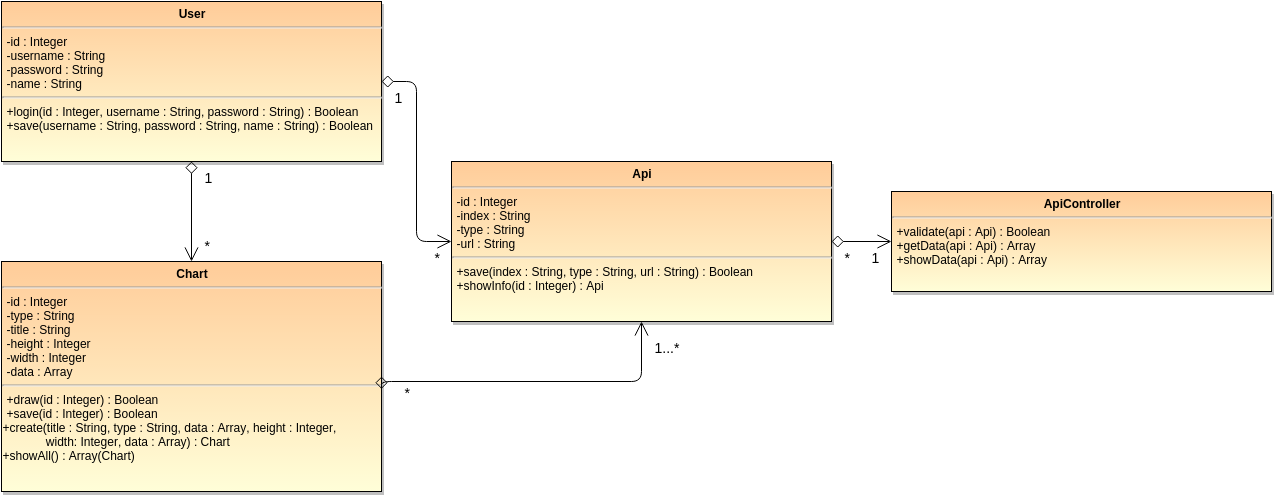
\includegraphics[scale=0.45]{Klassediagram}}
\caption{Klassediagram med relationer}
\label{fig:klassediagram}
\end{figure}
